\documentclass[letterpaper,twoside,12pt]{article}
\usepackage[dvips]{graphicx}
\usepackage[margin=0.8in]{geometry}
\usepackage{caption}
\usepackage{amsmath}
\usepackage{amssymb}
\usepackage[T1]{fontenc}
\usepackage{natbib}
\usepackage{authblk}
\bibliographystyle{agu08}

\newcommand{\ud}{\mathrm d}
\newcommand{\uj}{\mathrm{j}}
\newcommand{\bz}{\mathbf{z}}
\newcommand{\Real}{\mathrm{Re}}
\newcommand{\Imag}{\mathrm{Im}}
\newcommand{\dif}{\mathrm{d}}
\newcommand{\sigsig}{\sigma_1\sigma_2}
\newcommand{\varss}{\varsigma_1\varsigma_2}
\newcommand{\hvarss}{\hat{\varsigma}_1 \hat{\varsigma}_2}


\title{Normality Test for 2-bit Stream Data in Mark-5 Files}

\author[1]{L. V. Benkevitch}
\affil[1]{\small MIT Haystack observatory, Westford, MA 01886, USA.}


\begin{document}

\maketitle

\begin{abstract}
The radio astronomy data from a single dish are recorded in M5B (Mark-5) or VDIF formatted files. The recorded data are supposed to be Gaussian white noise. A corrupted data segment can be spotted at the output of correlation stage. However, the correlation is expensive and vastly increases the bulk of data to be analyzed for spurious parts. Here we consider a problem of finding non~Gaussian (or non-normal) single-dish data segments in M5B files.

The problem may be thought about from a security standpoint. Suppose someone (a malicious character) wishes to hack a system and figures an approach would be to embed some malicious code in. Is it possible to detect the embedded (non-Gaussian) data within a frame or multiple frames before the correlator? Also, even though an algorithm can be determined, is it possible to ensure its implementation is fast enough? The data files are large (up to a hundred gigabytes).

Our solution is based on Pearson's $\chi^2$ test. The null hypothesis states that the data in file  are consistent with the normal distribution. If the data in a part of the file do not pass the test at the significance level 0.05, the null hypothesis is rejected, and the data fragment is flagged.

The algorithm runs on the GPU (Graphics Processing Unit), which provides high speed computations.
\end{abstract}


\section{Quantization and M5B Data Structure}

The analog signal from a single antenna/dish is supposed to be Gaussian noise $N(\mu,\sigma)$ with the expectation $\mu$ and standard deviation (rms) $\sigma$ distributed according to the normal law with the probability density function (PDF):

\begin{equation}
  \label{normal_pdf}
  N(\mu,\sigma) =  \frac{1}{\sigma\sqrt{2\pi}} e^{-\frac{(x-\mu)^2}{2\sigma^2}}.
\end{equation}

The signal is centered to ensure zero $\mu$ and its band is filtered into 16 frequency channels each of which is passed through the 4-level quantizer with the characteristic shown in Fig.~\ref{quant4lvl}.  The quantizer has just three switching thresholds, $-\theta$, 0, and $\theta$, so it is characterized with the only parameter, the adjustable quantization threshold $\pm\theta$. Note that the hardware deals with voltage thresholds, $\pm v_0$, but $\theta$ is expressed in the signal STDs, thus it is dimensionless, $\theta = v_0/\sigma$. The quantizer output only takes four values as in Tab.~\ref{quant_io}. These values are saved in the M5B file.


\begin{figure}[h!]
  \begin{center}
  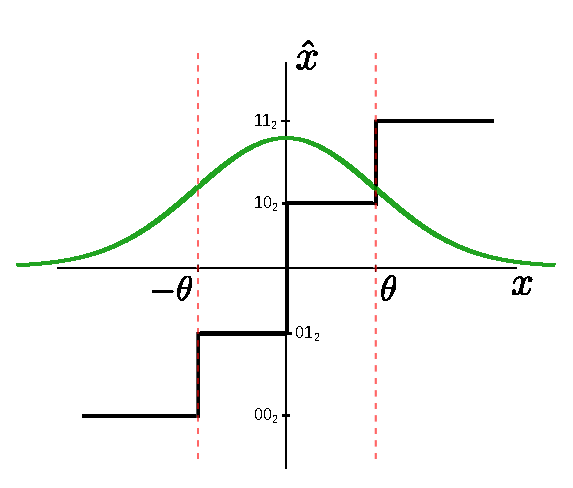
\includegraphics[width=25pc]{fig_4_Level_Quantization_Pattern_impr.eps}
  %\noindent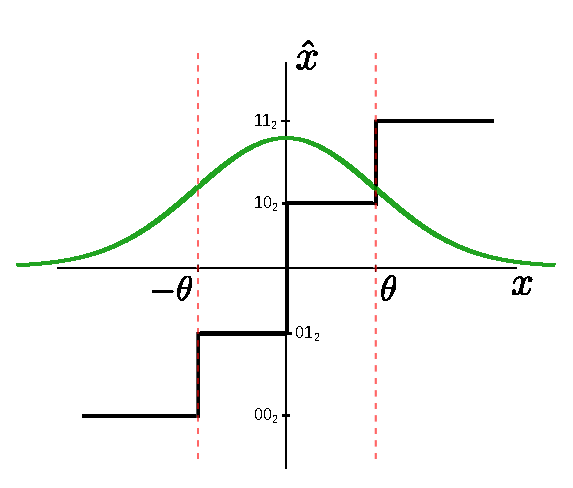
\includegraphics[width=20pc]{fig_4_Level_Quantization_Pattern_impr.eps}
  %\includegraphics[width=\linewidth]{}
  \caption{4-level quantization.}
  \label{quant4lvl}
  \end{center}
\end{figure}


\begin{table}[h!]
  \begin{center}
    \caption{Quantizer}
    \label{quant_io}
    \begin{tabular}{c|c}
      \textbf{Input} & \textbf{Output} \\
      \hline
      $-\infty$ to $-\theta$ & 0 \\
      $-\theta$ to 0         & 1 \\
      0 to $\theta$          & 2 \\
      $\theta$ to $+\infty$  & 3 \\
    \end{tabular}
  \end{center}
\end{table}


The M5B file can be considered as an array of 10016-byte frames. Each frame consists of 2504 32-bit words (\verb@unsigned int@ or  \verb@uint@ in C/C++). The first 4 words comprise the frame header, so a frame has 2500 words of pure data. Each 32-bit data word is subdivided into 16 2-bit channels, numbered from 0 to 15. 


Hereafter, we call $Q_i$ 



\section{ Data }




\end{document}



